% "{'classe':('PSI','PT'),'chapitre':'oral_mt','type':('oral_mt'),'titre':'Tête de découpe de tissus', 'source':'Concours Commun INP 2018 MP','comp':(),'corrige':False}"
%\setchapterimage{bandeau}
\chapter*{Préparation Mines Telecom \\%\arabic{cptColle} \\ 
Tête de découpe de tissus \ifnormal $\star$ \else \fi \iftdifficile $\star\star\star$ \else \fi  -- 
\ifprof Corrigé \else Sujet \fi}
\addcontentsline{toc}{section}{Colle \arabic{cptColle} :
Tête de découpe de tissus \ifnormal $\star$ \else \fi \iftdifficile $\star\star\star$ \else \fi  -- 
\ifprof Corrigé \else Sujet \fi}

\iflivret \stepcounter{cptColle} \else
\ifprof  \stepcounter{cptColle} \else \fi
\fi

\setcounter{question}{0}
\marginnote{D'après concours Commun INP 2018 -- MP.}
\marginnote{
\UPSTIcompetence[2]{}
}


\begin{marginfigure}
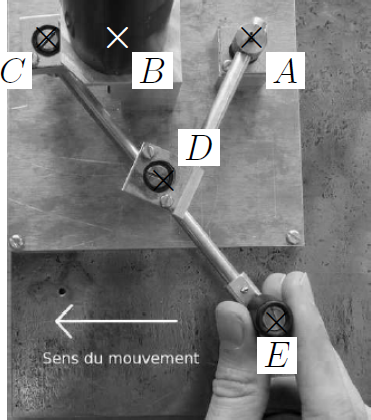
\includegraphics[width=\linewidth]{fig_00.png}
%\caption{Sous-système SEIS \label{fig_01}}
\end{marginfigure}


Le système étudié dans ce sujet est une tête de coupe de tissus conçue et réalisée par la société française Lectra, leader mondial dans la découpe automatisée des tissus.

\paragraph*{Présentation générale}

Un système de découpe automatisé de tissus est composé (figure \ref{fig_01}) :
\begin{itemize}
\item d’une table de découpe sur laquelle le tissus à découper (appelé matelas) est maintenu en position par aspiration ;
\item d’un bras transversal qui se déplace en translation de direction $\vy{0}$ par rapport à la table ;
\item d’une tête de coupe qui se déplace en translation de direction $\vx{0}$ par rapport au bras transversal ;
\item d’un ordinateur qui pilote l’ensemble du système.	 
\end{itemize}

\begin{marginfigure}
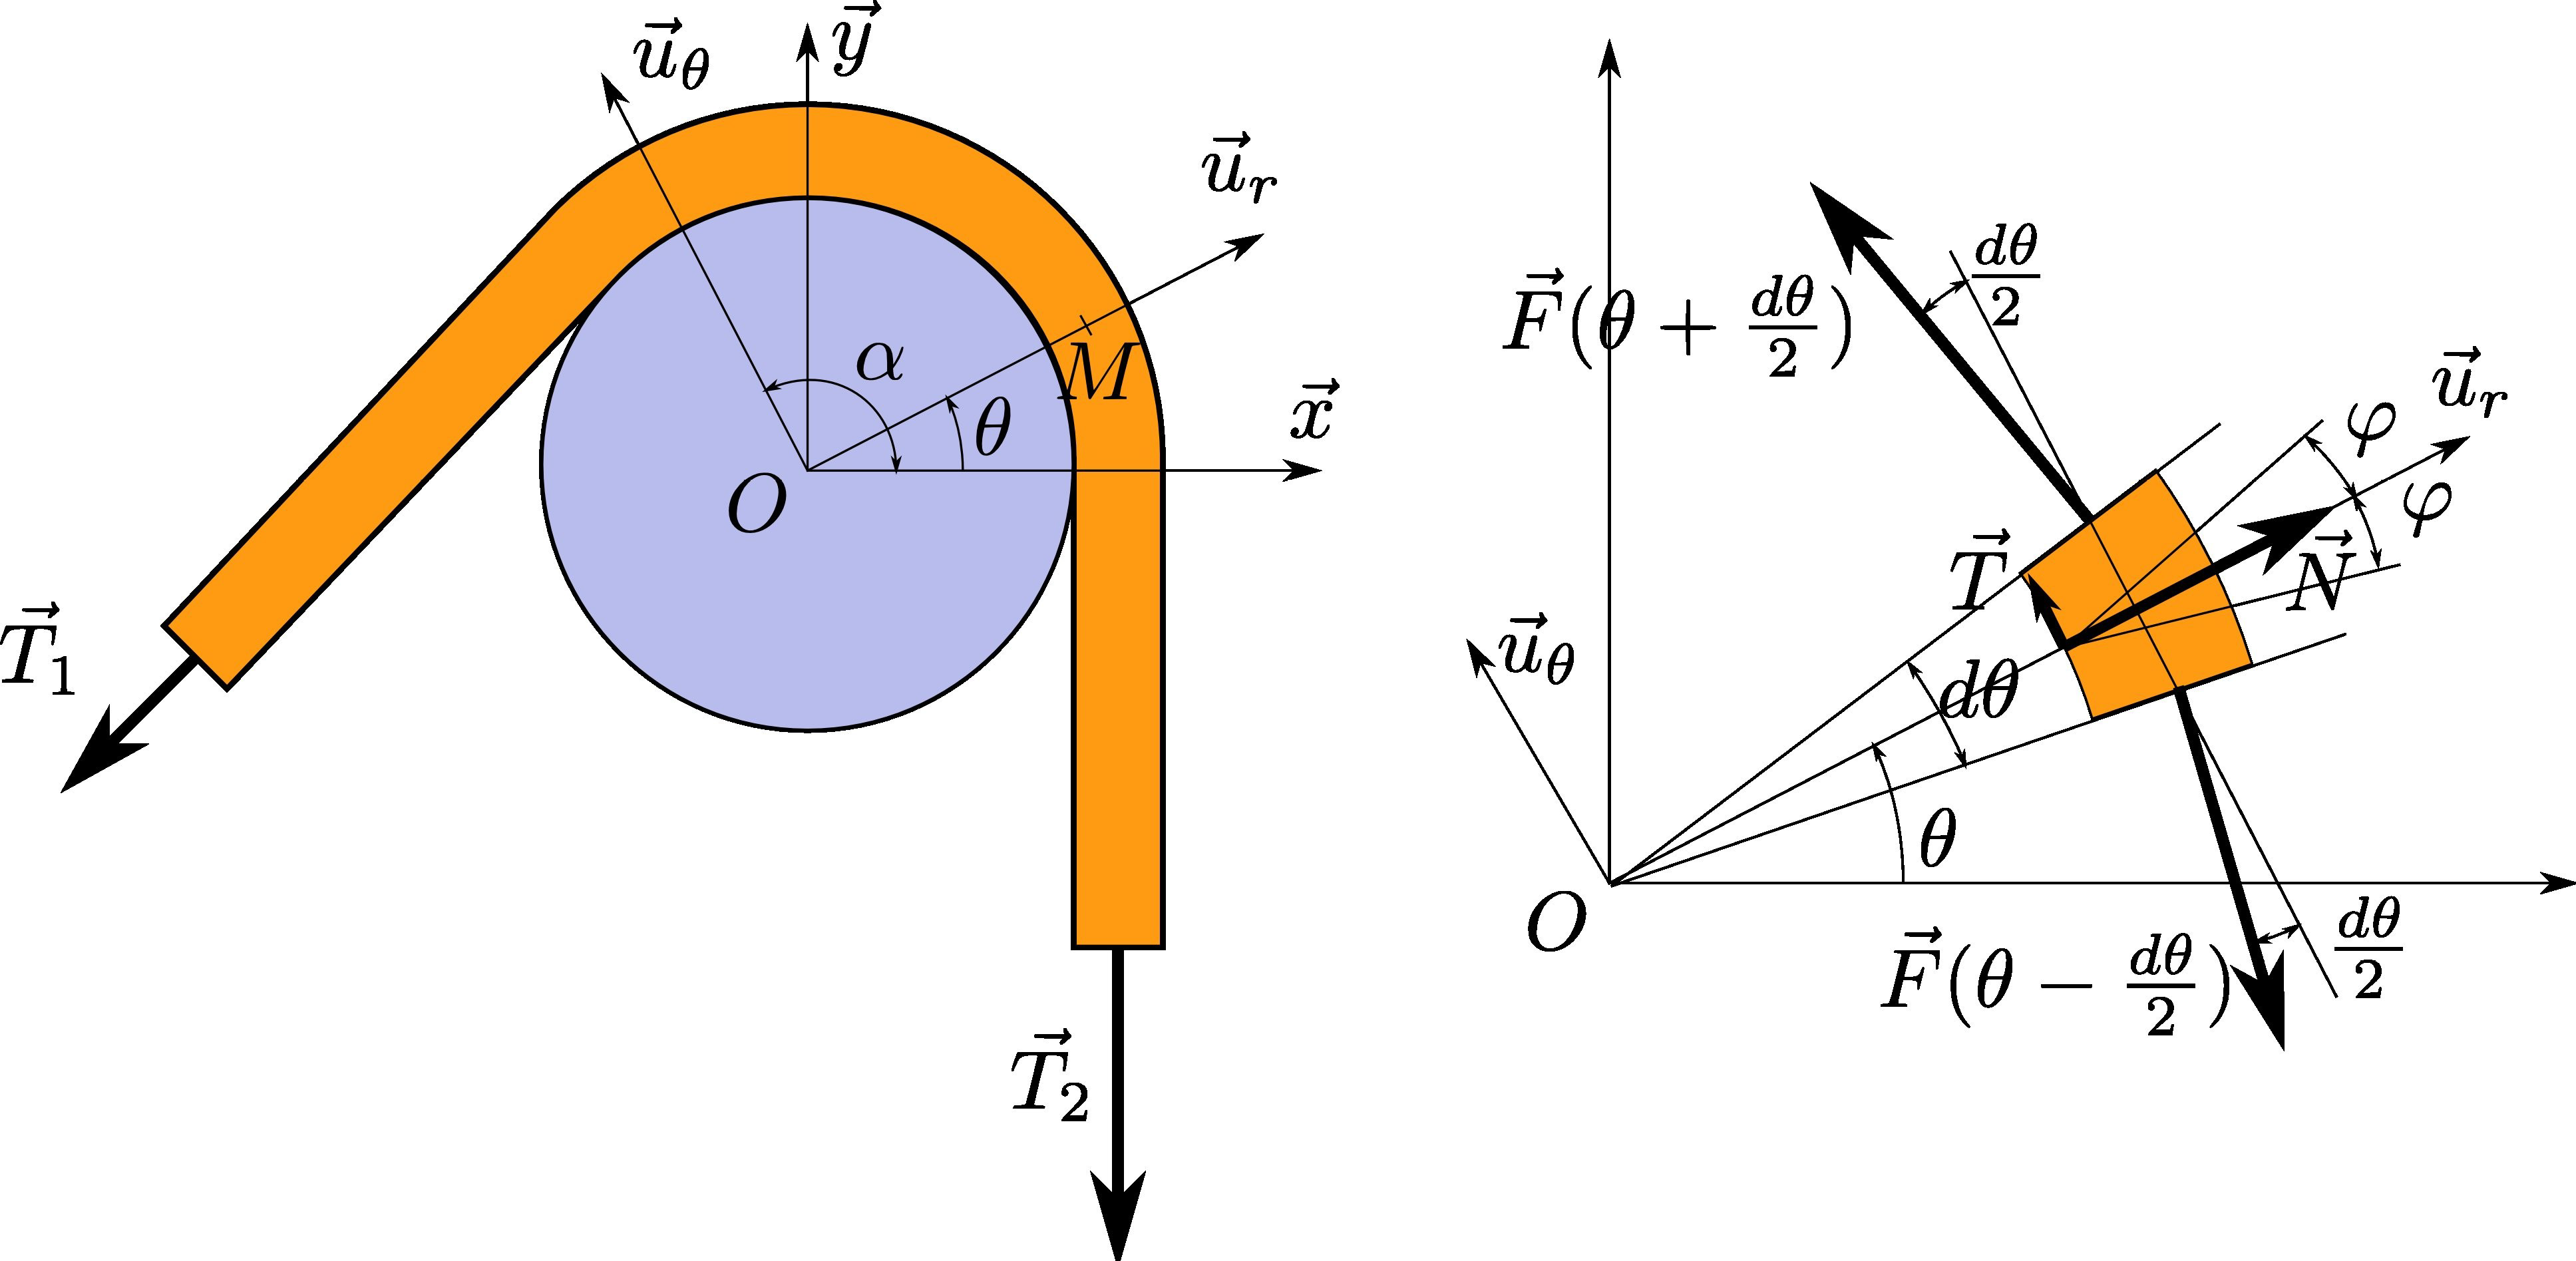
\includegraphics[width=\linewidth]{fig_01.png}
\caption{Structure d’une table de découpe de tissus \label{fig_01}}
\end{marginfigure}
	
Dans ce sujet, nous nous intéresserons plus particulièrement à la tête de coupe proposée par Lectra dans deux versions (initiale et améliorée) dont le diagramme partiel des exigences pour la solution de découpe (logiciel/machine) est présenté dans la figure~\ref{fig_02}.



\paragraph*{Modélisation du comportement cinématique de la tête de coupe}


\begin{marginfigure}
\centering
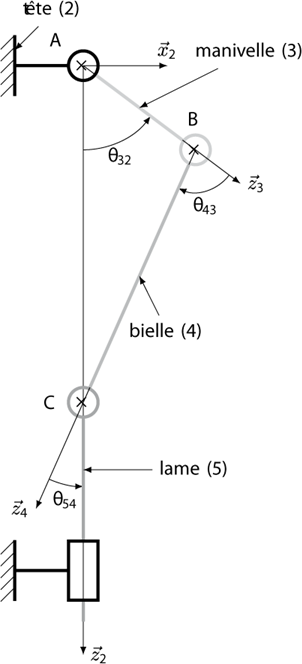
\includegraphics[width=\linewidth]{fig_09b.png}
\caption{Schéma cinématique  du système d’entraînement de la lame de coupe\label{fig_09}}
\end{marginfigure}


La découpe du tissu est réalisée par un mouvement de translation alternative d’une lame par rapport au matelas de tissus. Ce mouvement est obtenu par un système bielle-manivelle dont le schéma cinématique est donné par la figure 9. Les mouvements de translation de la tête de coupe par rapport à la table impliquent que les bases $\base{x_2}{y_2}{z_2}$ et $\base{x_0}{y_0}{z_0}$, liées respectivement à la tête de coupe et à la table, sont identiques (figure \ref{fig_01}).





\paragraph*{Modélisation des liaisons et paramétrage du système}

On associe le repère  $\rep{2}=\repere{A}{x_2}{y_2}{z_2}$ à la tête 2, le repère $\rep{3}=\repere{A}{x_3}{y_3}{z_3}$ à la manivelle 3, le repère $\rep{4}=\repere{B}{x_4}{y_4}{z_4}$ à la bielle 4 et le repère $\rep{5}=\repere{C}{x_5}{y_5}{z_5}$ à la lame 5.

La manivelle 3 est en liaison pivot avec la tête 2, d’axe $\axe{A}{y_2}$ et d’angle $\theta_{32} (t)= \angl{x_2}{x_3} = \angl{z_2}{z_3} $.

La manivelle 3 est en liaison pivot avec la bielle 4, d’axe $\axe{B}{y_2}$ et d’angle $\theta_{43} (t)= \angl{x_3}{x_4} = \angl{z_3}{z_5} $.

La bielle 4 est en liaison pivot avec la lame 5, d’axe $\axe{C}{y_0}$ et d’angle $\theta_{54} (t)= \angl{x_4}{x_2} = \angl{z_4}{z_2} $.

La lame 5 est en liaison glissière avec la tête 2, de direction  $\vz{2}$ et de paramètre linéaire $\lambda(t)$.
On pose $\omega_{ij} (t)= \dfrac{\dd \theta_{ij}}{\dd t} = \thetap_{ij}(t)$, $\vect{AB}=L_3\vz{3}$ avec $L_3=\SI{12,5}{mm}$, $\vect{BC}=L_4 \vect{z_4}$  avec $L_4=\SI{80}{mm}$ et $\vect{AC}=\lambda(t)\vz{2}$.


\begin{figure}
\centering
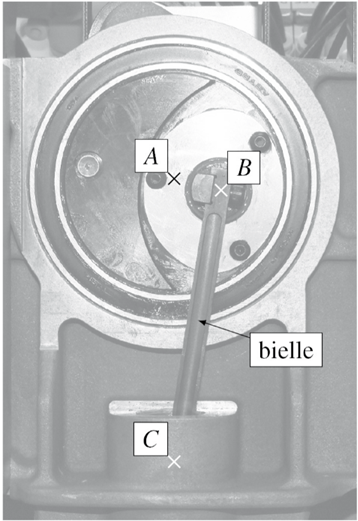
\includegraphics[width=.2\linewidth]{fig_09a.png}
\caption{Système d’entraînement de la lame de coupe}
\end{figure}

\begin{figure}
\centering
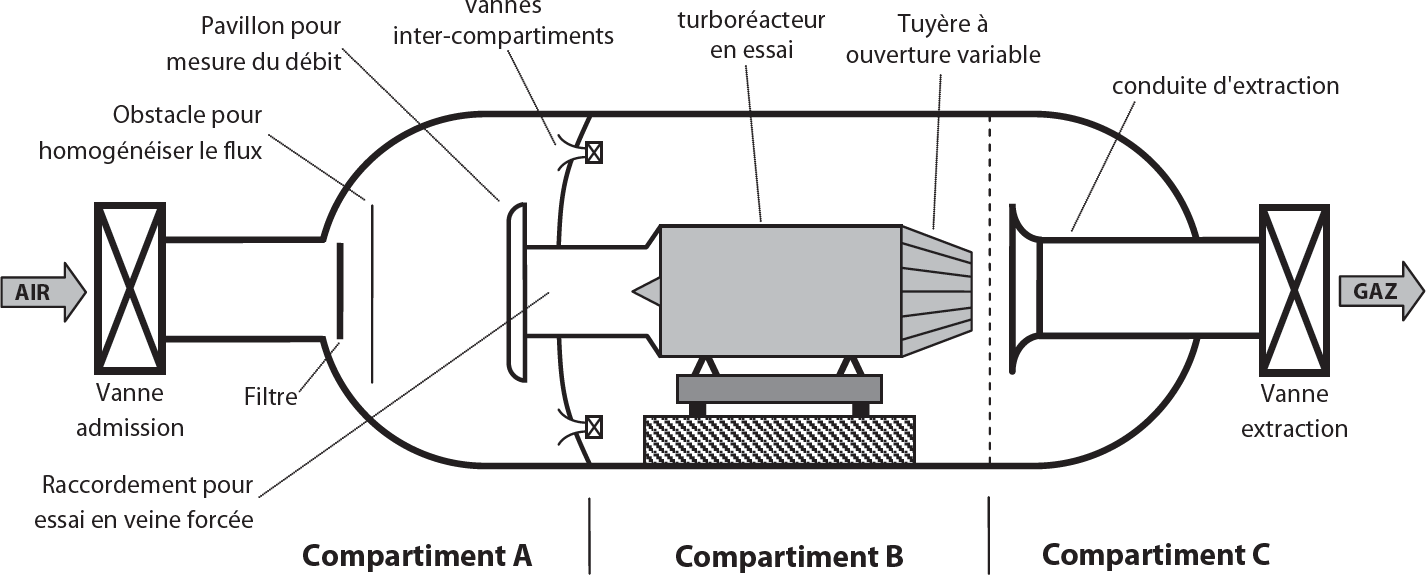
\includegraphics[width=\linewidth]{fig_02.png}
\caption{Diagramme des exigences \label{fig_02}}
\end{figure}
